\chapter{Probabilistic model checking}
We use Discrete-time Markov chain as the formalism to model stochastic population process. In this
chapter, we present essential concepts on probabilistic model checking, including probabilistic
models and properties. We also briefly present a general deterministic model checking algorithm for
a specific temporal logic, namely PCTL. Due to the state space explosion, applying deterministic
model checking algorithm is possible to be computationally expensive. Therefore, we also present a
simulation based model checking, namely \textit{statistical model checking} for bounded and
unbounded path property. Since statistical model checking relies only on simulation of stochastic
models, it is advantageous for checking models with large space size. We also introduce definitions
of parametric model and parameter synthesis problems, as well as the symbolic computing approach to
verify parametric models.


\section{Markov models}
\subsection{Discrete Time Markov chain}
Markov models are stochastic models of discrete or continous time which satisfy memoryless property.
\begin{definition}[Discrete-time memoryless property]
    Let $X$ be a random variable of geometric distribution. $X$ has memoryless property if and only if
    \begin{align*}
        Pr\{X = t + m | X > m\} = Pr\{X > m\} \forall t,m \in \mathbb{N} k \geq 1
    \end{align*}
\end{definition}
Markov model can be non-deterministic \textit{(Markov Decision Process)}. However, in this thesis we
consider only Markov models without non-determinism. The following definitions of discrete-time and
continuous-time Markov chains follows the definitions presented by Baier \cite{baier2008principles}.
\begin{definition}[Discrete Time Markov Chain]
    A Discrete-time Markov chain (DTMC) $\mathcal{M}$ is a tuple $(S,\mathbf{P}, \iota_{init}, AP, L)$,
    in which
    \begin{itemize}
        \item $S$ is a countable, non-emty set of \textit{states}
        \item $\mathbf{P}:S\times S \rightarrow [0,1]$ is the \textit{transition probability}
              function such that
              \begin{align*}
                  \forall s \in S : \sum_{s'\in S}\mathbf{P}(s, s') = 1
              \end{align*}
        \item $\iota_{init}: S \rightarrow [0,1]$ is the \textit{initial distribution} such that
              \begin{align*}
                  \sum_{s\in S} \iota_{init}(s) = 1
              \end{align*}
        \item $AP$ is a set of \textit{atomic propositions}.
        \item $L: S \rightarrow 2^{AP}$ is the labelling function on states.
    \end{itemize}
\end{definition}

\begin{example}[Knuth-Yao die]
    \begin{figure}[H]
        \centering
        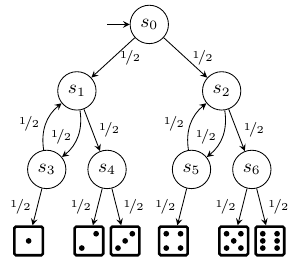
\includegraphics[width=0.5\textwidth]{figures/knuth_die.png}
        \caption{Knuth-Yao die to simulate a 6-faced die by a fair coin. Image taken from
            \cite{katoen2016probabilistic}}
        \label{fig:knuth-die}
    \end{figure}
\end{example}

\begin{definition}[Strongly Connected Component]
    Let $\mathcal{M}=(S,\mathbf{P}, \iota_{init}, AP,L)$ a DTMC. A subset $S'\subset S$ is strongly
    connected if and only if for every pair $s_1,s_2\in S'$ there is a path between $s_1$ and $s_2$
    which consists of only of state in $S'$. If there exist no $S''\subseteq S$, such that $S\subset
        S''$ and $S''$ is strongly connected, then $S'$ is a \textit{Strongly Connected Component}, or
    \textit{SCC} in short.
\end{definition}

\begin{definition}[Bottom Strongly Connected Component]
    Let $\mathcal{M}=(S,\mathbf{P}, \iota_{init}, AP,L)$ a DTMC and $S'\in S$ a Strongly Connected
    Component. $S'$ is also a \textit{Bottom Strongly Connected Component}, or \textit{BSCC} for
    short, if and only if there exist no state $s \in S\\S'$ that is reachable from any state in
    $S'$. If $|S'|=1$ then $S'$ is a \textit{trivial BSCC}. We denote $BSCC(\mathcal{M})\in S$ is
    the set of all BSCCs of $\mathcal{M}$.
\end{definition}
Intuitively, BSCCs are arbsobing; once a path in a DTMC reaches a state in a BSCC, it visits  all
states in the BSCC infinitely often. It is proven by \cite{baier2008principles} that any run on a
DTMC $\mathcal{M}$ ends in $BSCC(\mathcal{M})$ almost surely.
\begin{theorem}[Long-run theorem]
    Let $\mathcal{M}=(S,\mathbf{P}, \iota_{init}, AP,L)$ a DTMC.
    \begin{align*}
        P[\Diamond BSCC(\mathcal{M})] = 1
    \end{align*}
\end{theorem}

In this thesis we concern the \textit{steady-state distribution} of a DTMC.
\begin{definition}[Steady-state distribution]
    Let $\mathcal{M}=(S,\mathbf{P}, \iota_{init}, AP,L)$ a DTMC and vector $v_t$ be a transient state distribution
    \begin{align*}
        v_t = (P[X_t=s_1],\ldots,P[X_t=s_N]), s_0,\ldots,s_N \in S
    \end{align*}
    A transient state distribution $v$ of $\mathcal{M}$ is a steady-state distribution of $\mathcal{M}$ if and only if
    \begin{align*}
        v = vP
    \end{align*}
\end{definition}
As a result from long-run theorem, if $BSCC(\mathcal{M})\neq \emptyset$ then there exists a
steady-state distribution $v = (P[X=s_1],\ldots,P[X=s_{|S|}])$, such that
\begin{align*}
    \forall 1 \leq i \leq |S|: P[X=s_i] \neq 0 \Leftrightarrow s_i \in BSCC(\mathcal{M})
\end{align*}


\subsection{Continuous-time Markov chain}
The discrete-time memoryless property can also be extended into continuous-time memoryless property.
In continous-time, memoryless property has the following form
\begin{definition}[Continuous-time memoryless property]
    Let X be a continuous random variable of exponentially distribution. X has memoryless property
    if and only if
    \begin{align*}
        Pr\{X > t + \delta | X > t\} = Pr\{X > \delta\}, \forall t,\delta \in \mathbb{R}_{\geq 0}
    \end{align*}
\end{definition}
Based on continuous-time memory less property, we introduce the definition of \textit{Continous-time
    Markov chain} \cite{katoen2013model}.
\begin{definition}[Continuous-time Markov chain]
    A Continuous-time Markov chain (CTMC) $\mathcal{C}$ is a tuple $(S,\mathbf{P}, \mathbf{r}, \iota_{init}, AP, L)$
    \begin{itemize}
        \item $S$ is a countable, non-emty set of \textit{states}
        \item $\mathbf{P}:S\times S \rightarrow [0,1]$ is the \textit{transition probability}
              function such that
              \begin{align*}
                  \forall s \in S : \sum_{s'\in S}\mathbf{P}(s, s') = 1
              \end{align*}
        \item $\mathbf{r}:S \rightarrow \mathbb{R}_{>0}$ is the \textit{exit rate} function
              such that
              \begin{align*}
                  \forall s \in S : \sum_{s'\in S}\mathbf{P}(s, s') = 1
              \end{align*}
        \item $\iota_{init}: S \rightarrow [0,1]$ is the \textit{initial distribution} such that
              \begin{align*}
                  \sum_{s\in S}\iota_{init}(s) = 1
              \end{align*}
        \item $AP$ is a set of \textit{atomic propositions}
        \item $L: S \rightarrow 2^{AP}$ is the labelling function on states.
    \end{itemize}
\end{definition}

\begin{example}[CTMC]
    An example of a CTMC with 3 states.
    \begin{figure}[H]
        \centering
        \begin{tikzpicture}[->, >=stealth', auto, semithick, node distance=3cm]
            \tikzstyle{every state}=[fill=white,draw=black,thick,text=black]
            \node[initial, state, label=above:2]    (S0)                   {$S_0$};
            \node[state, label=above:4]    (S1)[right of=S0]      {$S_1$};
            \node[state, label=above:3]    (S2)[right of=S1]      {$S_2$};
            \path

            (S0)
            edge [bend left=20] node{$1$} (S1)

            (S1)
            edge [bend left=20] node{$\frac{2}{3}$} (S2)
            edge [bend left=20] node{$\frac{1}{3}$} (S0)

            (S2)
            edge [bend left=20] node{$1$} (S1);
        \end{tikzpicture}
        \label{fig:ctmc}
    \end{figure}
    \label{example:ctmc}
\end{example}

Continous-time Markov chain has a wide range of applications, especially in bioinformatics where
chemical reaction network \cite{feinberg1980chemical} \cite{anderson2011continuous}. However, the
frameworks in this thesis apply for discrete-time Markov models, thus we do not use continuous-time
Markov chain to model systems of interest directly. Instead, we do not use Continuous-time Markov
models directly. Instead, we transform CTMCs into DTMCs through uniformization \cite{katoen2016probabilistic}
\begin{definition}[CTMC Uniformization]
    Let $\mathcal{C} = (S,\mathbf{P}, \mathbf{r}, \iota_{init}, AP, L)$ be a CTMC. We define the
    \textit{uniformization rate} $r$ such that
    \begin{align*}
        \forall s\in S: r \geq \mathbf{r}(s), r\in\mathbb{R}_{>0}
    \end{align*}
    The \textit{uniformized CTMC} $unif(r, \mathcal{C})=(S, \bar{\mathbf{P}}, \bar{\mathbf{r}}, \iota_{init}, AP, L )$ such that
    \begin{align*}
        \forall s\in S     & : \bar{\mathbf{r}}(s)     \\
        \forall s, s'\in S & : \bar{\mathbf{P}}(s,s')=
        \begin{cases}
            \frac{\mathbf{r}(s)}{r}\mathbf{P}(s,s')                               & \text{if $s \neq s'$} \\ \quad \\
            \frac{\mathbf{r}(s)}{r}\mathbf{P}(s,s') + 1 - \frac{\mathbf{r}(s)}{r} & \text{if $s = s'$}
        \end{cases}
    \end{align*}
\end{definition}

\begin{example}[Uniformized CTMC]
    We uniformize the CTMC in Example \ref{example:ctmc} by uniformization rate $r=4$.
    \begin{figure}[H]
        \centering
        \begin{tikzpicture}[->, >=stealth', auto, semithick, node distance=3cm]
            \tikzstyle{every state}=[fill=white,draw=black,thick,text=black]
            \node[initial, state, label=above:4]    (S0)          {$S_0$};
            \node[state, label=above:4]    (S1)[right of=S0]      {$S_1$};
            \node[state, label=above:4]    (S2)[right of=S1]      {$S_2$};
            \path

            (S0)
            edge [bend left=20] node{$\frac{1}{2}$} (S1)

            (S1)
            edge [bend left=20] node{$\frac{2}{3}$} (S2)
            edge [bend left=20] node{$\frac{1}{3}$} (S0)

            (S2)
            edge [bend left=20] node{$\frac{3}{4}$} (S1);
        \end{tikzpicture}
        \label{fig:uniformized-ctmc}
    \end{figure}
\end{example}
It has been shown by Katoen \cite{katoen2013model} that uniformization preserves the transient
probability distributions. Furthermore, in this thesis we concern steady state data and state
property, thus uniformizing exit rate does not affect the validity of our constructed frameworks.

\section{Property specification}
\subsection{Probabilistic Computational Tree Logic}
Model checking verifies a formalism of a system \textit{(model)} against a property of interest. We
formalize a property by a \textit{temporal logic}, specifically \textit{Probabilistic Computational
    Tree Logic} (or \textit{PCTL}). Firstly introduced by Clarke et al. \cite{clarke1986automatic}, PCTL
is widely used in model checking of discrete-time stochastic models and supported by most
probabilistic model checking tools \cite{dehnert2017storm}, \cite{kwiatkowska2011prism}.
\begin{definition}[PCTL] The syntax of PCTL consists of state formulas and path formulas.
    \begin{itemize}
        \item State formulas are defined over $AP$
              \begin{align*}
                  \Phi & ::== \text{true} \;|\; a \;|\; \Phi \;|\; \Phi_1 \wedge \Phi_2 \;|\; \Phi_1 \vee \Phi_2 \;|\;  P_{J}[\phi]
              \end{align*}
              where $a\in AP$, $\phi$ is a path formula, and $J\subseteq[0,1]$ is an interval.
        \item Path formulas
              \begin{align*}
                  \phi & ::== \bigcirc \Phi \;|\; \Phi_1 \mathsf{U} \Phi_2 \;|\; \Phi_1 \mathsf{U}^{\leq n} \Phi_2
              \end{align*}
              where $\Phi,\Phi_1,\Phi_2$ are state formulas, and $n\in \mathbb{N}$.
    \end{itemize}
\end{definition}
PCTL properties is applicable on discrete-time stochastic models such as DTMC, as the times between
state transitions are uniform. In a DTMC, a PCTL state formula is verified at each state, while a
PCTL path formula is verified through a trace from an execution path.
\begin{example}

\end{example}

\subsection{Model checking PCTL properties}
Given a DTMC $\mathcal{M}$ and a PCTL property $\Phi$, general algorithm for checking
$\mathcal{M}\models\Phi$ consists of the following steps:

\begin{algorithm}[H]
    \caption{Model checking a DTMC against a PCTL}
    \label{alg:dtmc-model-checking}
    \begin{algorithmic}[1]
        \Procedure{Dtmc-Check-Pctl}{}
        \EndProcedure
    \end{algorithmic}
\end{algorithm}

\begin{theorem}[Complexity of checking a DTMC against a PCTL formula.]

\end{theorem}
\subsection{State exlosion problem}
The soundness of the model checking relies heavily on how the system is modeled. In fact, the model
checking is only as sound and valid as the model.
\begin{enumerate}
    \item Which formalism is used?
    \item How the system is encoded into states and transitions?
\end{enumerate}
Consider a distributed software system, in which a \textit{global state} is a composition of
\begin{itemize}
    \item values of all variables, and
    \item states of all communication channels.
\end{itemize}
It is obvious that the number of possible states grows exponentially as


\section{Statistical Model checking}
Statistical model checking is a simulation-based approach to model check a stochastic model
$\mathcal{M}$ against a temporal property $\Phi$. The essential concept of probabilistic model
checking is to simulate traces from $\mathcal{M}$, verify if each trace satisfies $\Phi$, then
estimate probability $P(\mathcal{M}\models\Phi)$ by a statistical, frequentist approach.
\subsection{Statistical model checking of unbounded properties.}
Estimation method, Chernoff-Hoeffding bound.
\begin{algorithm}[H]
    \caption{APMC Statistical Model Checking}
    \label{alg:smc-apmc}
    \begin{algorithmic}[1]
        \Procedure{SMC-APMC}{}
        \EndProcedure
    \end{algorithmic}
\end{algorithm}

\subsection{Statistical model checking of bounded properties.}

\begin{algorithm}[H]
    \caption{SPRT Statistical Model Checking}
    \label{alg:smc-sprt}
    \begin{algorithmic}[1]
        \Procedure{SMC-SPRT}{}
        \EndProcedure
    \end{algorithmic}
\end{algorithm}

\section{Parametric model}
We introduce parameters to formalize unknown attributes of the system.
\begin{definition}[Polynomial ring]
    Given a tuple $\mathbf{x}=(x_1,\ldots,x_n)$ be a tuple
\end{definition}

\begin{definition}{Rational functions}
    Let $\mathbf{x}=\{x_1,\ldots,x_n\}$ be a variable; let $\mathbf{Pol}[\mathbf{x}]$ be the set of
    all polynomial functions over $\mathbf{x}$. A rational function $h(\mathbf{x})$ is defined
    as following.
    \begin{align*}
        h(x) := \frac{f(\mathbf{x})}{g(\mathbf{x})}, f,g\in\mathbf{Pol}[\mathbf{x}], g(\mathbf{x}) \neq 0
    \end{align*}
    We denote $\mathbb{Q}(\mathbf{x})$ the set of all rational functions over $\mathbf{x}$.
\end{definition}


\subsection{Parametric Discrete Time Markov chain}
With the set of rational functions formally defined, we define parametric Discrete-time Markov chain
based the definition on \cite{junges2019parameter}.
\begin{definition}[Discrete Time Markov Chain]
    A Discrete-time Markov chain (DTMC) is a tuple $(S, \mathbf{x}, \mathbf{P}, \iota_{init}, AP, L)$
    where
    \begin{itemize}
        \item $S$ is a countable, non-emty set of \textit{states}
        \item $\mathbf{x} \in \mathbb{R}^n, n \in \mathbb{N}$ as the set of $n$ real parameters.
        \item $\mathbf{P}:S\times S \rightarrow \mathbb{Q}(\mathbf{x})$ is the \textit{transition
                  probability} function such that
              \begin{align*}
                  \forall s \in S : \sum_{s'\in S}\mathbf{P}(s, s') = 1
              \end{align*}
        \item $\iota_{init}: S \rightarrow [0,1]$ is the \textit{initial distribution} such that
              \begin{align*}
                  \sum_{s\in S}\iota_{init}(s) = 1
              \end{align*}
        \item $AP$ is a set of \textit{atomic propositions}
        \item $L: S \rightarrow 2^{AP}$ is the labelling function on states.
    \end{itemize}
\end{definition}

\begin{example}[Parametric Knuth-Yao die]
    A Knuth-Yao die to simulate a 6-faced die by two unfair coins with probability of one
    side $p$ and $q$. Image taken from \cite{katoen2016probabilistic}.
    \begin{figure}[H]
        \centering
        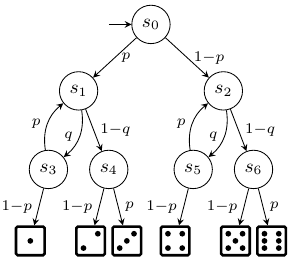
\includegraphics[width=0.5\textwidth]{figures/knuth_die_pq.png}
        \label{fig:knuth-die-pq}
    \end{figure}
\end{example}

Given a parametric Discrete-time Markov chain $\mathcal{M}_\theta$. A concrete assignment of parameter $\theta$
\textit{instantiates} a non-parametric Discrete-time Markov chain if $f{\theta}$ evaluates to a
real value for all $f\in\mathbf{P}$.

\subsection{Symbolic model checking of pDTMC}

\begin{example}{Parametric Knuth's die}
    We continue the example with Knuth die model $\mathcal{M}_{p}$. Assume the
    \begin{align*}
        x =
    \end{align*}
\end{example}

\subsection{Parameter synthesis of pDTMC}

\begin{example}
    Given a pDTMC of Knuth die $\mathcal{M}_{p}$ and a path property $\Phi = P_{\geq 0.2} [F
                \texttt{"one"}]$, synthesize parameter $p$ so that $\mathcal{M}_{p} \models \Phi$. A simple
    Monte-Carlo search on parameter space gives the following satisfying point:
    %% Figures
\end{example}

